\documentclass[a4paper, 12pt, titlepage]{article}
\usepackage[utf8]{inputenc}
\usepackage{geometry}
\usepackage{polski}
\usepackage{graphicx}
\usepackage{float}
\usepackage{etoolbox,refcount}
\usepackage{multicol}
\usepackage{tabularx}

\newgeometry{left=2cm, right=2cm, bottom=2cm, top=2cm}
\title{Dokumentacja testów -- Sygnalizacja świetlna}
\author{Adrian Jałoszewski, Tomasz Kotowski \\ Dorota Kowalik, Michał Krent}
\date{}

\begin{document}
	\maketitle
	\tableofcontents
	\newpage
	\section{Testy włączeń}
		\subsection{Włączenie pierwszego cyklu}
			Działa poprawnie:
			\begin{figure}[H]
				\centering
				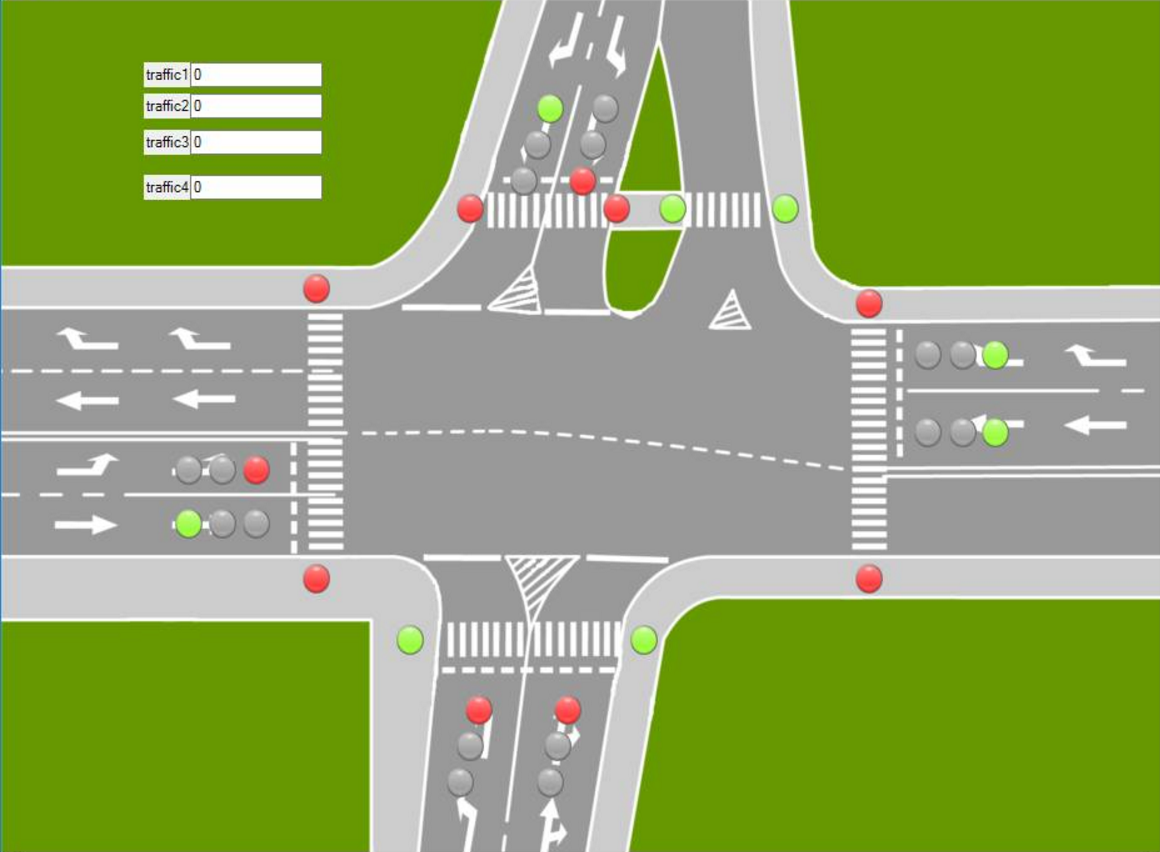
\includegraphics[height=0.4\textheight]{./img/pierwszy.png}
			\end{figure}
		\subsection{Włączenie drugiego cyklu}
			Działa poprawnie:
			\begin{figure}[H]
				\centering
				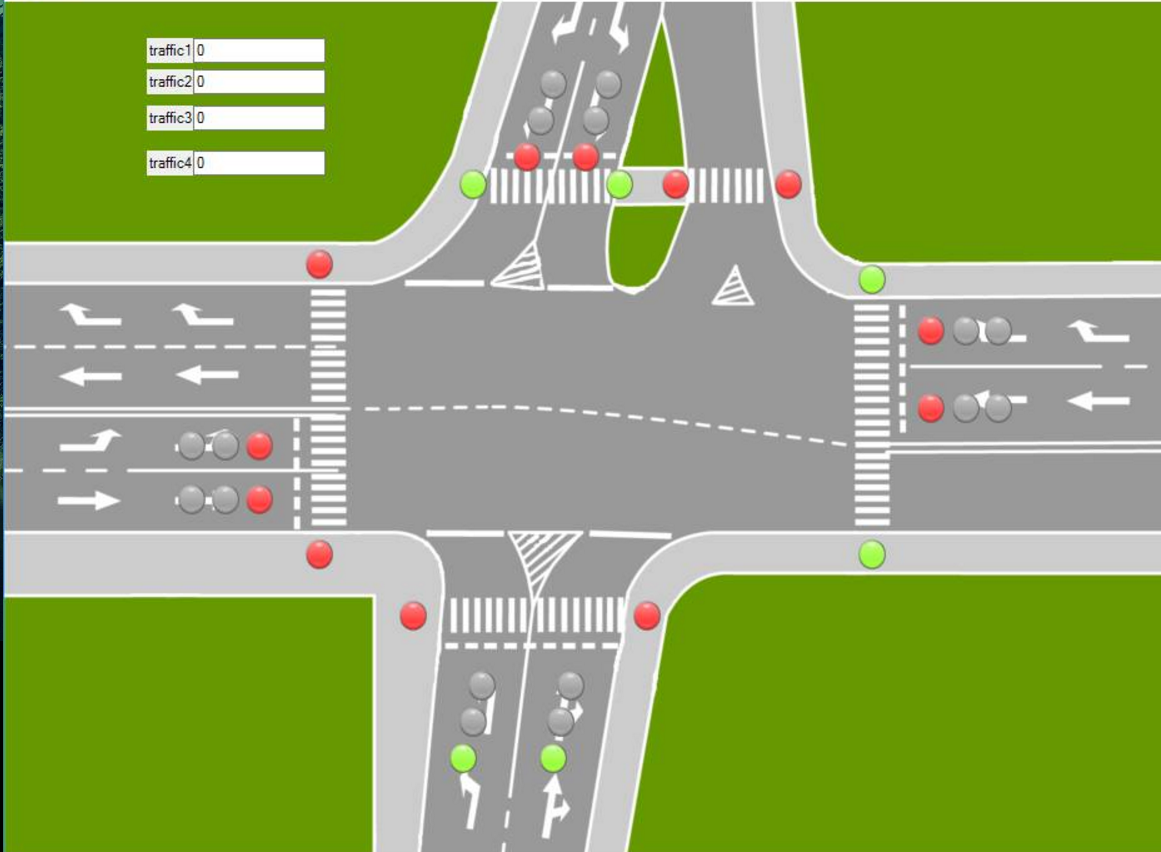
\includegraphics[height=0.35\textheight]{./img/drugi.png}
			\end{figure}
		\subsection{Włączenie trzeciego cyklu}
			Działa poprawnie:
			\begin{figure}[H]
				\centering
				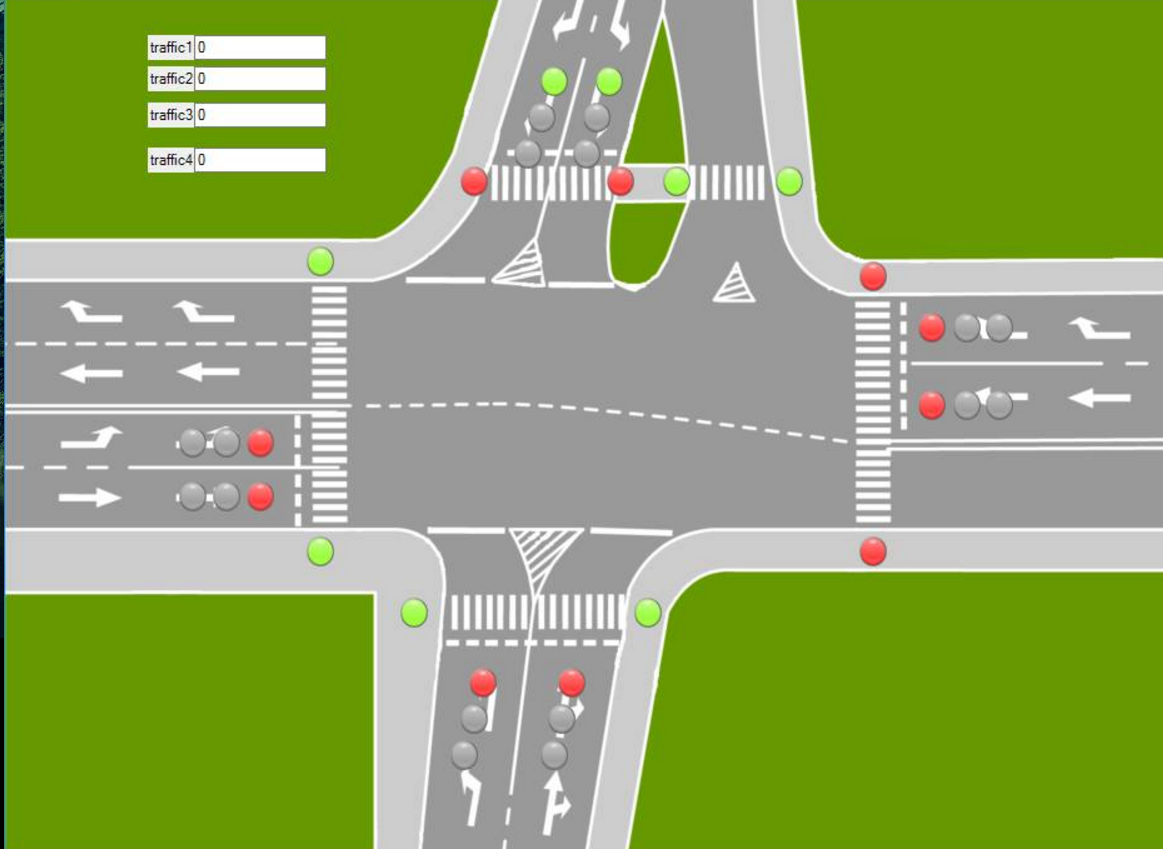
\includegraphics[height=0.35\textheight]{./img/trzeci.png}
			\end{figure}
		\subsection{Włączenie czwartego cyklu}
			Działa poprawnie:
			\begin{figure}[H]
				\centering
				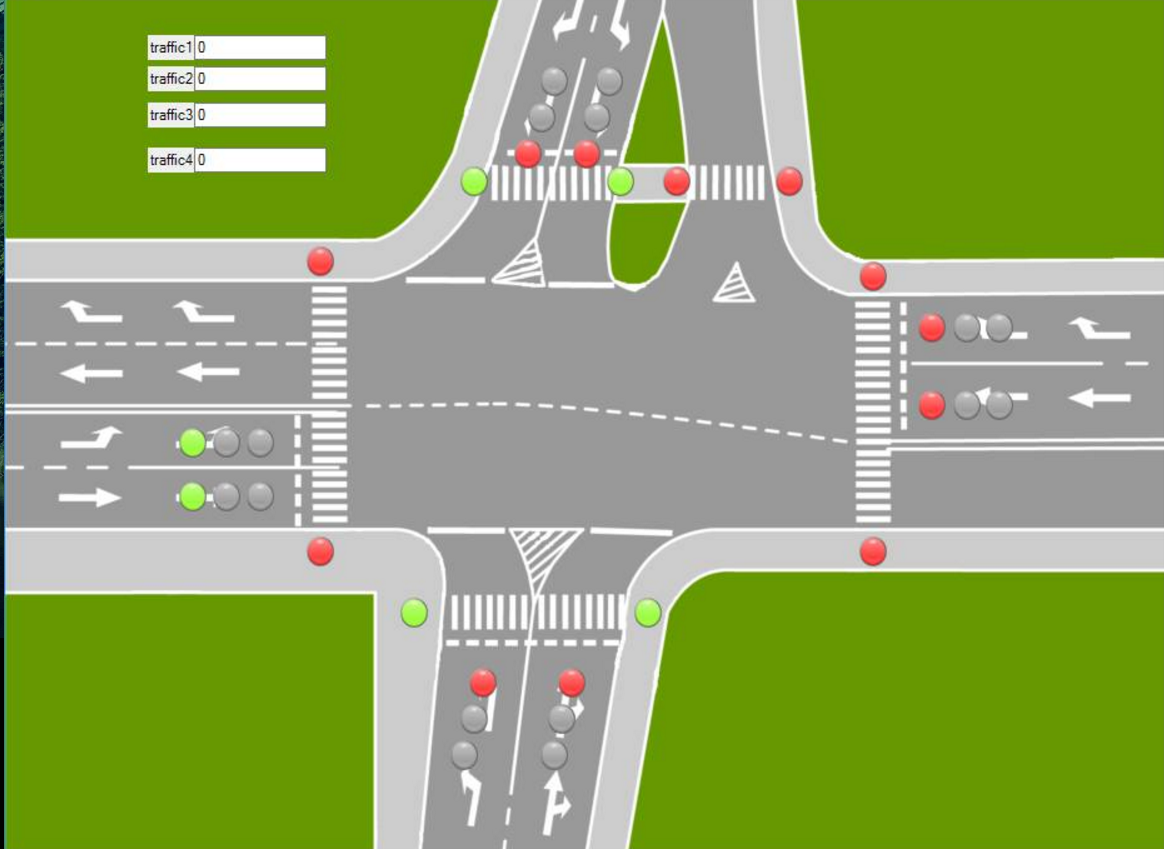
\includegraphics[height=0.35\textheight]{./img/czwarty.png}
			\end{figure}
	\newpage
	\section{Testy przełączeń}
		\subsection{Z pierwszego}
			\subsubsection{Do pierwszego}
				Działa poprawnie:
				\begin{itemize}
					\item[--] zielone -- podtrzymane
					\item[--] czerwone -- podtrzymane
					\item[--] przejścia -- podtrzymane
				\end{itemize}
			\subsubsection{Do drugiego}
				Działa poprawnie:
				\begin{itemize}
					\item[--] żółte--czerwone -- ustawione
					\item[--] żółte -- ustawione
					\item[--] przejścia -- czerwone
					\item[--] pozostałe czerwone -- podtrzymane
				\end{itemize}
			\subsubsection{Do trzeciego}
				Działa poprawnie:
				\begin{itemize}
					\item[--] zielone, te same -- podtrzymane
					\item[--] żółte--czerwone -- ustawione
					\item[--] żółte -- ustawione
					\item[--] przejście, te same -- podtrzymane
					\item[--] pozostałe czerwone -- podtrzymane
					\item[--] pozostałe przejścia -- czerwone
				\end{itemize}
			\subsubsection{Do czwartego}
				Działa poprawnie:
				\begin{itemize}
					\item[--] zielone, te same -- podtrzymane
					\item[--] żółte--czerwone -- ustawione
					\item[--] żółte -- ustawione
					\item[--] przejście, te same -- podtrzymane
					\item[--] pozostałe czerwone -- podtrzymane
					\item[--] pozostałe przejścia -- czerwone
				\end{itemize}
		\newpage
		\subsection{Z drugiego}
			\subsubsection{Do pierwszego}
				Działa poprawnie:
				\begin{itemize}
					\item[--] żółte--czerwone -- ustawione
					\item[--] żółte -- ustawione
					\item[--] przejścia -- czerwone
					\item[--] pozostałe czerwone -- podtrzymane
				\end{itemize}
			\subsubsection{Do drugiego}
				Działa poprawnie:
				\begin{itemize}
					\item[--] zielone -- podtrzymane
					\item[--] czerwone -- podtrzymane
					\item[--] przejścia -- podtrzymane
				\end{itemize}
			\subsubsection{Do trzeciego}
				Działa poprawnie:
				\begin{itemize}
					\item[--] wszystkie przejścia -- czerwone
					\item[--] żółte--czerwone -- ustawione
					\item[--] żółte -- ustawione
					\item[--] pozostałe czerwone -- podtrzymane
				\end{itemize}
			\subsubsection{Do czwartego}
				Działa poprawnie:
				\begin{itemize}
					\item[--] wspólne przejście -- podtrzymane
					\item[--] żółte--czerwone -- ustawione
					\item[--] żółte -- ustawione
					\item[--] pozostałe czerwone -- podtrzymane					
				\end{itemize}
				\newpage
		\subsection{Z trzeciego}
			\subsubsection{Do pierwszego}
				Działa poprawnie:
				\begin{itemize}
					\item[--] zielone, te same -- podtrzymane
					\item[--] żółte--czerwone -- ustawione
					\item[--] żółte -- ustawione
					\item[--] przejście, te same -- podtrzymane
					\item[--] pozostałe czerwone -- podtrzymane
					\item[--] pozostałe przejścia -- czerwone
				\end{itemize}
			\subsubsection{Do drugiego}
				Działa poprawnie:
				\begin{itemize}
					\item[--] wszystkie przejścia -- czerwone
					\item[--] żółte--czerwone -- ustawione
					\item[--] żółte -- ustawione
					\item[--] pozostałe czerwone -- podtrzymane
				\end{itemize}
			\subsubsection{Do trzeciego}
				Działa poprawnie:
				\begin{itemize}
					\item[--] zielone -- podtrzymane
					\item[--] czerwone -- podtrzymane
					\item[--] przejścia -- podtrzymane
				\end{itemize}
			\subsubsection{Do czwartego}
				Działa poprawnie
				\begin{itemize}
					\item[--] wspólne przejście -- podtrzymane
					\item[--] żółte--czerwone -- ustawione
					\item[--] żółte -- ustawione
					\item[--] pozostałe czerwone -- podtrzymane
				\end{itemize}
				\newpage
		\subsection{Z czwartego}
			\subsubsection{Do pierwszego}
				Działa poprawnie:
				\begin{itemize}
					\item[--] zielone, te same -- podtrzymane
					\item[--] żółte--czerwone -- ustawione
					\item[--] żółte -- ustawione
					\item[--] przejście, te same -- podtrzymane
					\item[--] pozostałe czerwone -- podtrzymane
					\item[--] pozostałe przejścia -- czerwone
				\end{itemize}
			\subsubsection{Do drugiego}
				Działa poprawnie:
				\begin{itemize}
					\item[--] wspólne przejście -- podtrzymane
					\item[--] żółte--czerwone -- ustawione
					\item[--] żółte -- ustawione
					\item[--] pozostałe czerwone -- podtrzymane					
				\end{itemize}
			\subsubsection{Do trzeciego}
				Działa poprawnie
				\begin{itemize}
					\item[--] wspólne przejście -- podtrzymane
					\item[--] żółte--czerwone -- ustawione
					\item[--] żółte -- ustawione
					\item[--] pozostałe czerwone -- podtrzymane
				\end{itemize}
			\subsubsection{Do czwartego}
				Działa poprawnie:
				\begin{itemize}
					\item[--] zielone -- podtrzymane
					\item[--] czerwone -- podtrzymane
					\item[--] przejścia -- podtrzymane
				\end{itemize}
				\newpage
	\newpage
	\section{Testy wyłączania bloczków}
		Testy te zostały przeprowadzone poprzez wprowadzenie tymczasowych dyrektyw wypisujących informację na ekran.
		\subsection{Pierwszy}
			Bloczek drugi przejął rolę pierwszego w zmianie świateł, trzeci bloczek aktualizuje globalne czasy.
		\subsection{Drugi}
			Bloczek pierwszy zmienia światła, trzeci bloczek aktualizuje globalne czasy.
		\subsection{Trzeci}
			Bloczek pierwszy zmienia światła, drugi bloczek aktualizuje globalne czasy.
		\subsection{Pierwszy i drugi}
			Trzeci bloczek pracuje sam, wykonując zadania pierwszego i swoje.
		\subsection{Pierwszy i trzeci}
			Drugi bloczek pracuje sam, wykonując zadania pierwszego i trzeciego.
		\subsection{Drugi i trzeci}
			Pierwszy bloczek pracuje sam, wykonując zadania swoje i trzeciego.
		\subsection{Wszystkie działają}
			Pierwszy bloczek odpowiada za przełączanie świateł, drugi jest na wypadek jakby któryś przestał działać, trzeci aktualizuje globalne czasy.
	\newpage
	\section{Testy funkcjonalności}
		\subsection{Zmiana wartości natężenia}
			Układ reaguje w każdym cyklu na nowe ustawienia i poprawnie dobiera następny element.
		\subsection{Skrzyżowanie puste lub natężenia te same}
			Układ zmierza do stabilizacji w trybie stałoczasowym.
		\subsection{Duży ruch w jednym cyklu}
			Układ przepuszcza na najbardziej zatłoczonym cyklu i wybiera ten cykl jako kolejny do chwili kiedy kryterium czasu oczekiwania nie będzie odgrywało głównej roli.
		\subsection{Bardzo duży ruch}
			Ograniczniki zastosowane w obliczeniach nie pozwalają na przekroczenie maksymalnej wartości zmiennej i zwrócenie prze funkcje do timerów ujemnych czasów.
		\subsection{Długotrwała praca układu}
			Układ dzięki odpowiednio pod to dobranych czasów synchronizacji nie posiada przypadków wyścigów przez co układ działa zgodnie z oczekiwaniami.
		\subsection{Awaria sterowników w chwili przełączania świateł}
			Na wypadek takiej sytuacji, której jednak nie byliśmy w stanie przesymulować w CANoe mamy przed każdą zmianą świateł resetowane ustawienia -- światła na chwilę niezauważalną dla ludzkiego oka (kilka obliczeń na bloczku) są ustawiane na kolor czerwony. W takiej sytuacji w razie jakby sterownik przełączając światła uległ awarii, to albo trwa poprzedni cykl dalej, albo z poprzedni cykl z zablokowanymi niektórymi torami pojazdów, albo wszystkie światła są zablokowane -- nie dochodzi do kolizji.
\end{document}